\documentclass[11pt,letterpaper,oneside,notitlepage]{article}	% specify paper type/format

\newcommand{\pd}[2]{\frac{\partial #1}{\partial #2}}	% partial derivative
\newcommand{\tensor}{\overleftrightarrow}		% tensor command
\newcommand{\del}{\vec\nabla}				% Del operator
\newcommand{\dop}{\tensor{\mathcal{D}}}		% Divergence operator (contrived)
\newcommand{\flux}{\tensor{\mathcal{G}}}		% Flux operator (contrived)
\newcommand{\yestag}{\tag{\theequation}\stepcounter{equation}}	% tags an equation number in the align* structure
\newcommand{\eq}[1]{Equation \eqref{#1}}		% Formated equation command

\setlength{\parindent}{6mm}  					% paragraph indent size
\newcommand{\pindent}[1]{\hspace{6mm}}  		% first paragraph indent size (match value with \parindent)
\linespread{1} 		     						% set spacing for entire paper
										% 1.6 is double spacing, 1 is single spaced
\usepackage{setspace}						% Allows me to set entire document spacing
\usepackage{amsmath}						% Needed for tensor symbol \overleftrightarrow{}
\usepackage{graphicx}						% Allows figures to be plotted
\usepackage{subfigure}						% Make multiple images in one figure
\numberwithin{equation}{section}				% Makes equation number relative to section

\begin{document}							% above = preamble, below = document

\title{Support Operator Method applied to a tensor diffusion coefficient on a regular, orthogonal grid\\ {\small Notes based primarily on Runnels' 2006 LANL Technical Report and Morel's 1998 SOM paper}}
\author{Nick Patterson}
\date{\today}								% sets date
\maketitle									% compiles title, author, and date

%\newpage
\tableofcontents
\newpage

%%%%%%%%%%%%%%%%%%%%%%%%%%%%%%%%%%%%%%%%%%%%%%%%%%%%
\section{Introduction and Scope of This Paper}%%%%%%%%%%%%%%
\pindent{}The Support Operator Method (SOM) is simply a means of discretizing a differential equation problem such that important properties of the continuum problem are maintained in the discrete form. While there are many interpretation of that statement and many forms that the SOM can take, this paper shows all the details necessary to derive and implement the SOM for a 2D, orthogonal grid with a tensor diffusion coefficient. While the orthogonal grid (Cartesian) case has more simple and easier to implement methods that can be used to solve the equation, the SOM is important for its flexibility. Having an SOM code for the diffusion equation allows for a non-scalar diffusion coefficient as well as having general quadrilaterals instead of rectangles or even shapes with more or less than four sides, such as triangles or pentagons. Also, this method will naturally handle the `hanging node' problem frequently created when using Adaptive Mesh Refinement (AMR). Whatever the grid type that one ends up using, the SOM will set up a matrix equation to be solved with a Symmetric Positive-Definite (SPD) coefficient matrix. Furthermore, this same method can be expanded to 3D, orthogonal or not, and it will still have a SPD coefficient matrix. The details shown here are only for the 2D, orthogonal case, but with the references cited and work shown here, only slight modifications to the set up are necessary to add this flexibility. 

The SOM discretization takes place in two steps\cite{Lipnikov2004}. The first step discretizes the integral relationship for a single cell in the mesh, taking into account the contribution from the diffusion equation as well. This is the local system, which only needs the values in the center of the cell and an the center of each face. The second step connects the equations for each cell such that concentration is continuous and the normal component of the flux is continuous across each face of each cell. This is the global step, which forms the coefficient matrix that is sent to the iterative solver.

%%%%%%%%%%%%%%%%%%%%%%%%%%%%%%%%%%%%%%%%%%%%%%%%%%%%
\section{Integral Identity}%%%%%%%%%%%%%%
\pindent{}To begin with the derivation of the Support Operator Method, only two things are needed: the divergence theorem and the chain rule.  The divergence theorem can be stated as follows,
\begin{equation}
\int_V \del\cdot\vec\xi\ dV = \oint_{\partial V} \vec \xi \cdot \hat n\ dA \label{DivThm},
\end{equation}
where $\vec \xi$ is any arbitrary vector, $V$ is the volume of interest, $\partial V$ is the boundary of the volume, $\hat n$ is the outward unit normal, and $A$ is the surface area of the boundary.  The other equation of interest comes from the application of the chain rule to the product of an arbitrary scalar function, $\phi$, and an arbitrary vector function, $\vec H$.  The following series of steps show the straightforward development of the equation of interest:
\begin{align}
\del\cdot(\phi\vec H) &= \phi(\del\cdot\vec H) + \vec H\cdot\del\phi \\
\int_V\del\cdot(\phi\vec H)\ dV &= \int_V\left(\phi(\del\cdot\vec H) + \vec H\cdot\del\phi\right)dV \\
\oint_{\partial V}(\phi\vec H)\cdot\hat n\ dA &= \int_V\phi\del\cdot\vec H\ dV + \int_V\vec H\cdot\del\phi\ dV \label{ConsEq}.
\end{align}
The second step applies a volumetric integral, and the last step applies \eq{DivThm} for $\vec\xi=\phi\vec H$.  This identity, \eq{ConsEq}, holds true for sufficiently smooth, arbitrary functions $\phi$ and $\vec H$ in a volume $V$\cite{Runnels2006}.

To apply \eq{ConsEq} to the solution of the discretized diffusion equation, define the volume $V$ to be one cell in a 2D orthogonal mesh, and $\partial V$ to be the perimeter of each cell.  The mesh will have regular spacings of $\Delta x$ in the x-direction and $\Delta y$ in the y-direction, giving $V$ a value of $\Delta x\ \Delta y$.  Note that in 2D, the `volume' is an area while in 3D it is an actual volume, $\Delta x\ \Delta y\ \Delta z$.

The diffusion equation is written as
\begin{equation}
\pd{\phi}{t}-\del\cdot(\tensor D \del \phi) = q,
\end{equation}
where $\phi$ is the concentration, $\tensor D$ is the diffusion tensor, and $q$ is a source/sink function.  Flux is defined as,
\begin{align}
\vec F &= -\tensor D\del\phi \label{FluxDef}.
\end{align}
Note that the diffusion tensor is assumed to be invertible. Using this new definition, the diffusion equation becomes,
\begin{equation}
\pd{\phi}{t}+\del\cdot\vec F = q\label{DifEq}.
\end{equation}
\eq{ConsEq} can be applied specifically to this application substituting \eq{FluxDef} into the last term, becoming
\begin{equation}
\oint_{\partial V}(\phi\vec H)\cdot\hat n\ dA = \int_V\phi\del\cdot\vec H\ dV - \int_V\vec H\cdot\tensor D^{-1}\vec F\ dV\label{IntId},
\end{equation}
where the superscript $-1$ represents the matrix inverse. Just to be completely clear, note that for arbitrary vector and tensor function, $\vec H\cdot\tensor G\vec F \neq \tensor G\vec H\cdot\vec F$, which can be shown trivially.

We now must discretize \eq{IntId} because it contains the differential properties that we want our operators to contain as well.  Note that this equation is another form of the Hilbert space relation which can show that the two operators in the SOM are adjoint, which is a more mathematical formulation of the SOM and based on Hyman's papers \cite{Hyman1997, Hyman1998, Hyman2002, Hyman2004}.  Also note that by construction, \eq{IntId} automatically enforces the relationship between flux and concentration, \eq{FluxDef}. 

%%%%%%%%%%%%%%%%%%%%%%%%%%%%%%%%%%%%%%%%%%%%%%%%%%%%
\section{Discretization of a Cell}%%%%%%%%%%%%%%
\pindent{}The integral relation must be discretized over a single arbitrary cell. For ease of notation, let us define a vector J such that
\begin{equation}
\vec J = \tensor D^{-1}\vec F \label{DefJ}.
\end{equation}
Then the integral relation is 
\begin{equation}
\oint_{\partial V}(\phi\vec H)\cdot\hat n\ dA = \int_V\phi\del\cdot\vec H\ dV - \int_V\vec H\cdot \vec J\ dV\label{IntID}.
\end{equation}
The assumption is that each cell is homogeneous, but variables can vary from cell to cell\cite{Morel1998}.  The location of the data points for an arbitrary cell (i,j) is shown in Figure \ref{Fig-Labels-Layout}.  Cell (i,j) is defined by the nodes (i,j), (i+1,j), (i+1,j+1), and (i,j+1).  The cell-centered concentration is denoted as $\phi^c$, while the face-centered concentrations are denoted as $\phi^T, \phi^R, \phi^B,$ and $\phi^L$, depending of if the value in question is on the top, right, bottom, or left side of the cell.  Similarly, an arbitrary vector $\vec H$ is defined for cell (i,j) on the faces as $h^T, h^R, h^B,$ and $h^L$.

\begin{figure}[ht]
\centering		% centers figure on page, instead of hugging left edge
\subfigure[Layout of cell (i,j) in a 2D mesh where nodes, cell faces, and the cell center are clearly labeled.]{\label{Fig-Cell-Layout}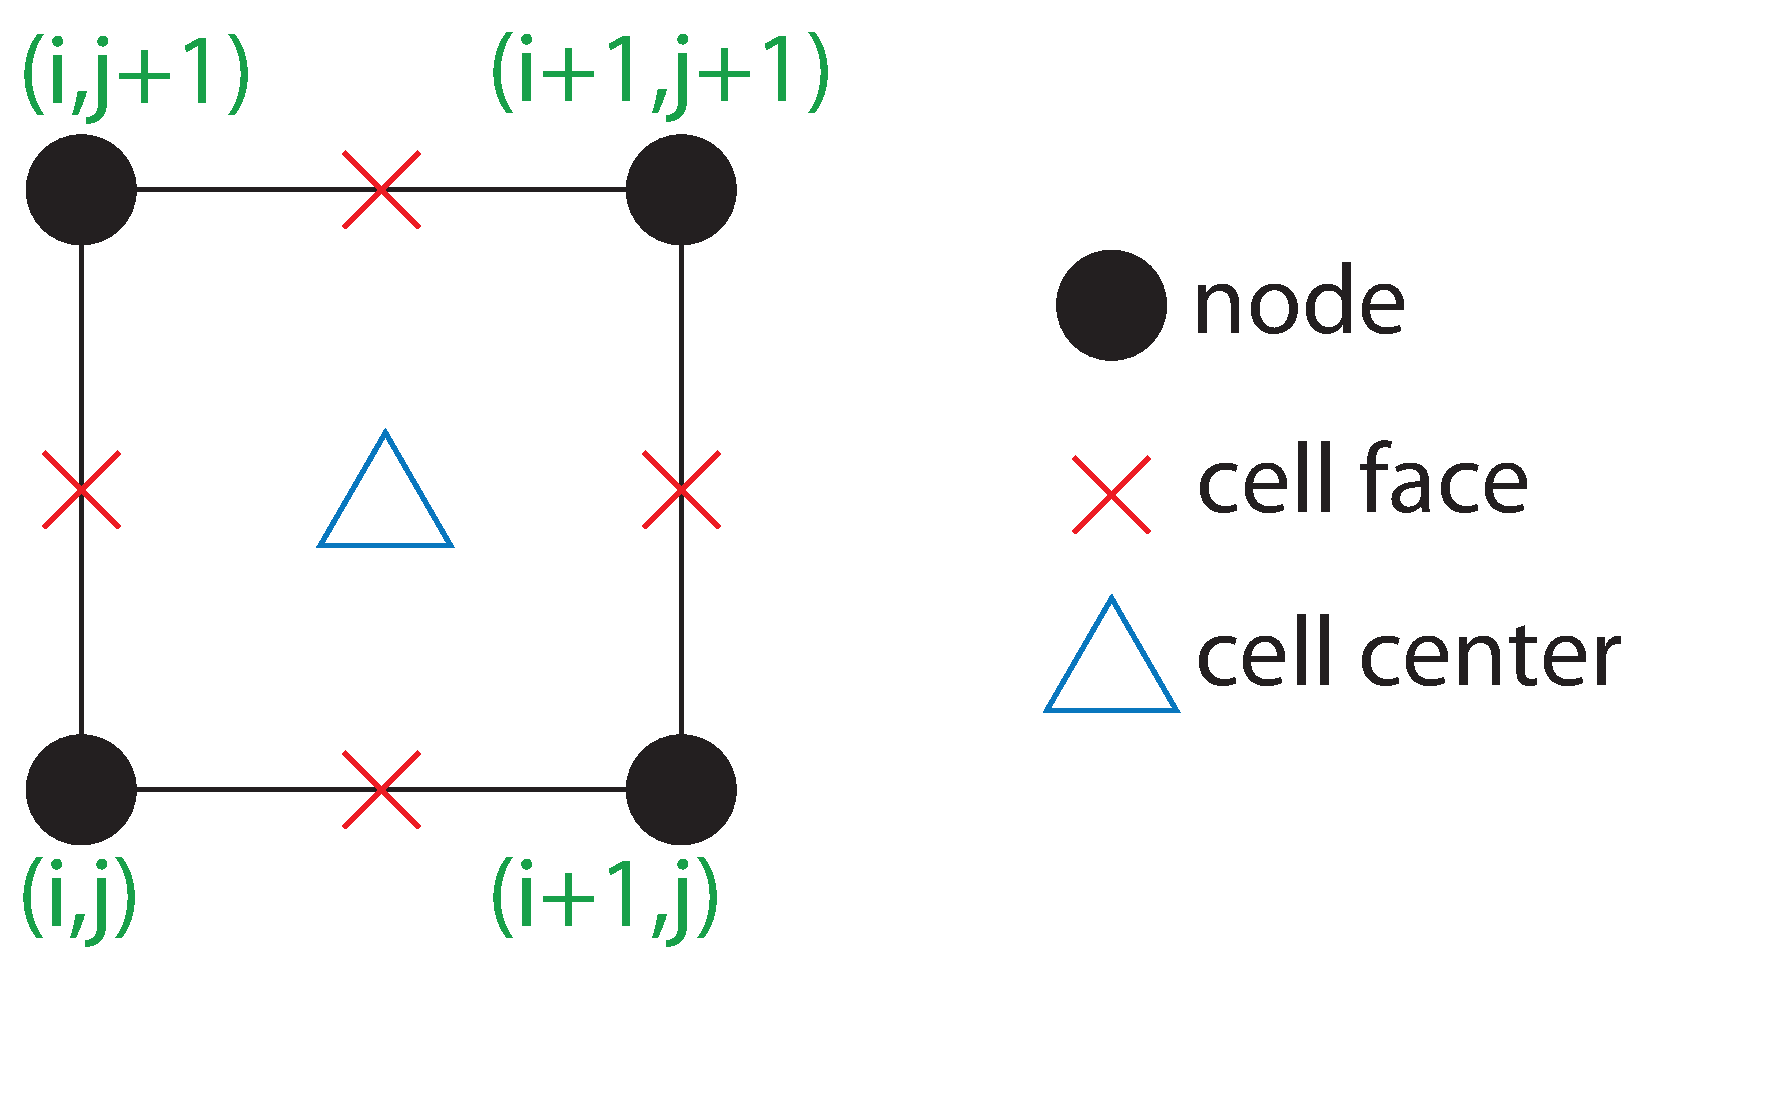
\includegraphics[height=1.5in]{Fig-Labels-2D}}
\subfigure[Location of vector components, which are face-centered for each cell's surface. Figure derived from Morel 1998\cite{Morel1998}]{\label{Fig-Cell-Vector}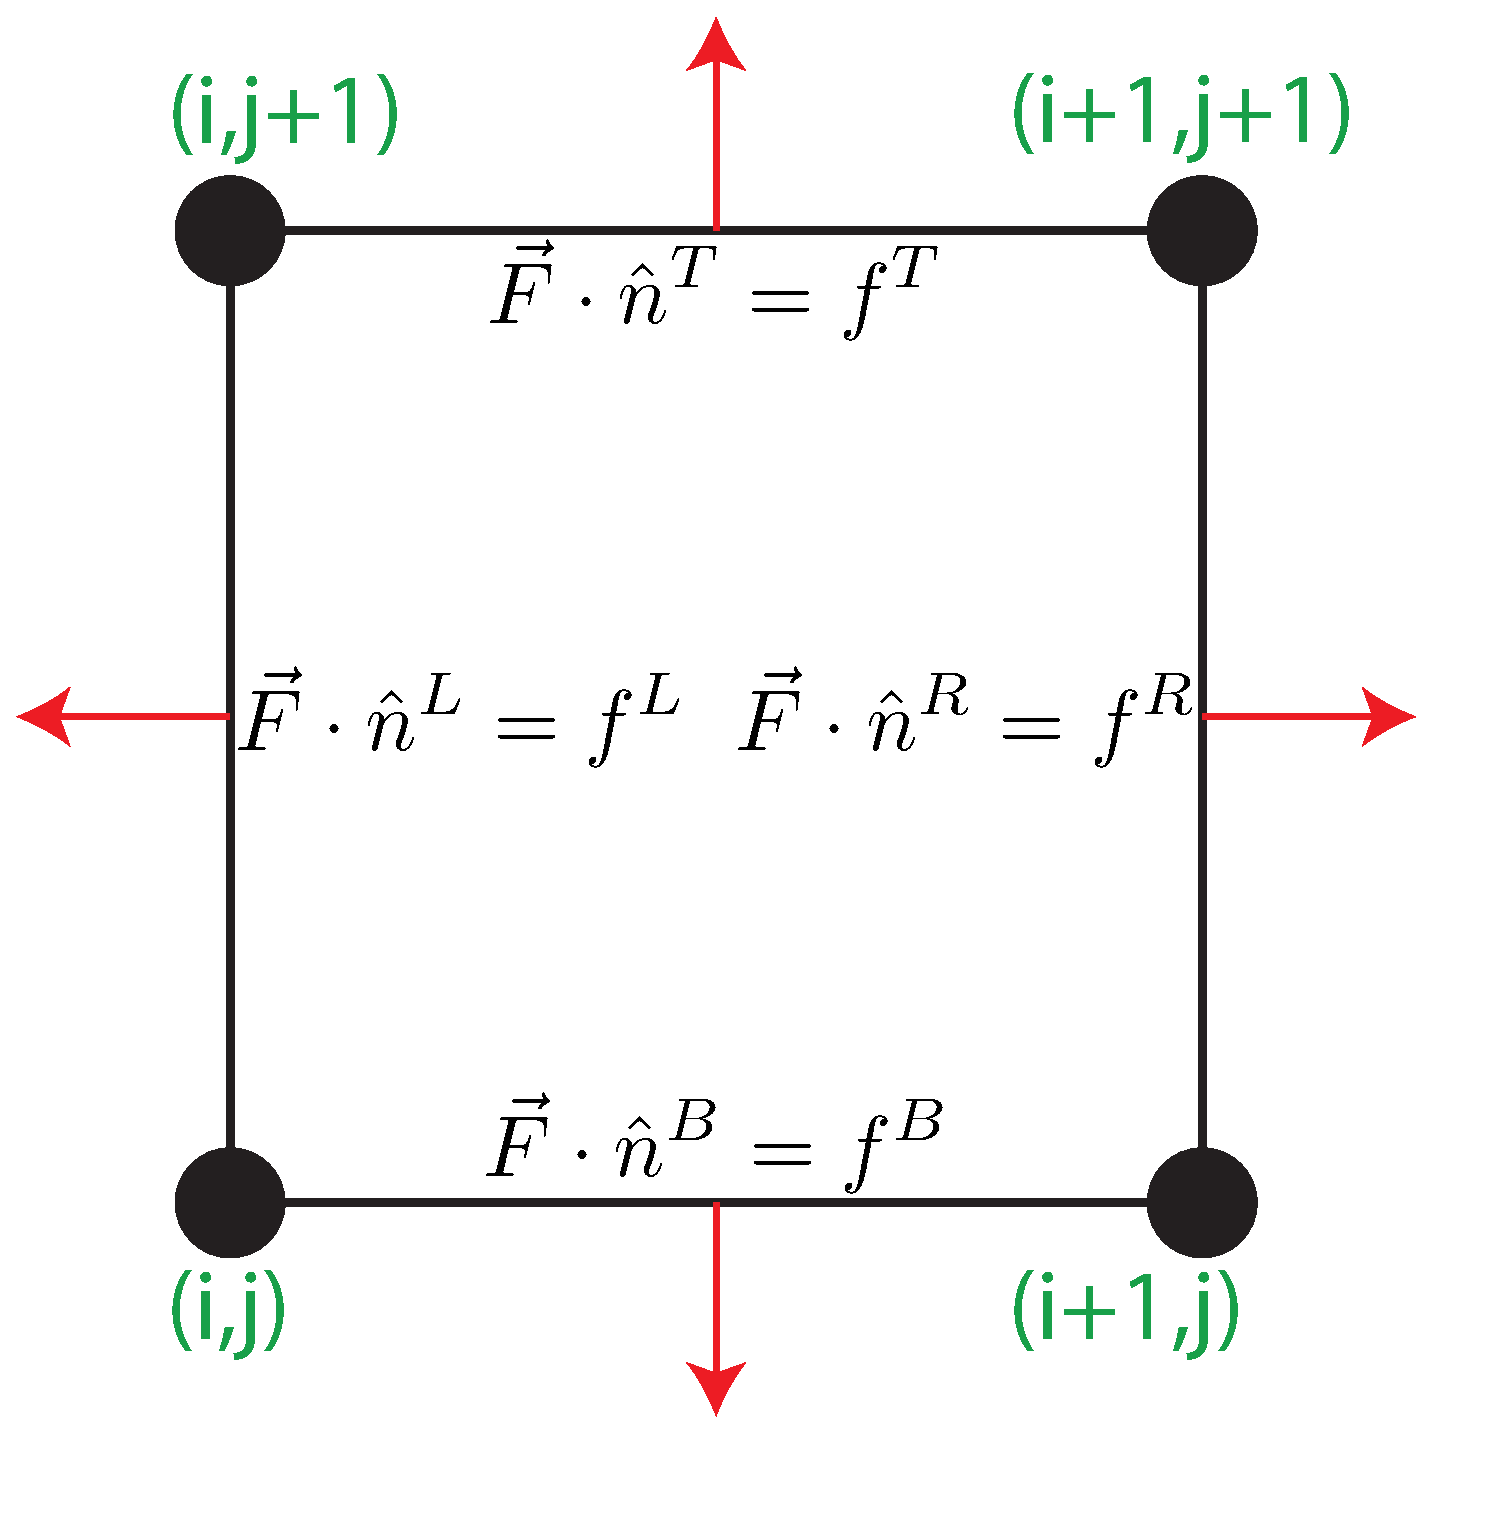
\includegraphics[height=1.5in]{Fig-Labels-Vector}}
\caption{Coordinates of the mesh and location of data.  These four nodes define cell (i,j). The concentration, $\phi$, is located at cell-center.  Also, there exists concentration values on each cell-face, which is where the vector-components are stored as well.}
\label{Fig-Labels-Layout}
\end{figure}

Now we begin to systematically make approximations of the continuous integrals with discrete summations.  We begin with the left-hand side term of \eq{IntID}, $\oint_{\partial V}(\phi\vec H)\cdot\hat n\ dA$.  The signs of $\vec H\cdot\hat n$ are embedded in the components, $h^\alpha$, see Figure \ref{Fig-Cell-Vector}, which means every term in the expression will be positive.  Hence, we can make the approximation that
\begin{equation}
\oint_{\partial V}(\phi\vec H)\cdot\hat n\ dA \approx \Delta y (\phi^R h^R + \phi^L h^L) + \Delta x (\phi^T h^T + \phi^B h^B)\label{Disc1a},
\end{equation}
where the area of the cell in our 2D case for $\hat n = \hat x$ is $\Delta y$ and for $\hat n = \hat y$ is $\Delta x$.  Note that any vector with a hat ($\hat \alpha$) is a unit vector.   
Recall that this integral came from the divergence theorem, so we know that 
\begin{equation}
\oint_{\partial V}(\phi\vec H)\cdot\hat n\ dA = \int_V \del\cdot(\phi \vec H)\ dV.
\end{equation}
If we wish to discretize the right-hand side, we have the following:
\begin{align}
\notag\int_V \del\cdot(\phi \vec H)\ dV &\approx \Delta x\  \Delta y\left[\frac{\phi^R h^R + \phi^L h^L}{\Delta x} + \frac{\phi^T h^T +\phi^B h^B}{\Delta y}\right] \\
&= \Delta y (\phi^R h^R + \phi^L h^L) + \Delta x (\phi^T h^T + \phi^B h^B)\label{Disc1b}.
\end{align}
Note that \eq{Disc1b} is identical to \eq{Disc1a}, which shows that the discrete divergence theorem is valid in these particular approximations.

The next term to discretize is $\int_V\phi\del\cdot\vec H\ dV$.  Since $\phi$ is being multiplied by the divergence of $\vec H$, and the divergence of a vector is a scalar, the components of $\phi$ are not needed, only the cell-centered value.  Since this value, $\phi^C$, is constant throughout the cell, it is constant in the integral, giving $\phi^C\int_V\del\cdot\vec H\ dV $.  This leads to the following discretization,
\begin{equation}
\int_V\phi\del\cdot\vec H\ dV \approx \phi^C\left[ \Delta y (h^R + h^L) + \Delta x (h^T + h^B)\right]\label{Disc2}.
\end{equation}

The remaining term, $\int_V\vec H\cdot\vec J\ dV$, can be approximated similarly. Each term will be multiplied by its volume fraction, which for us will simply be $\frac{\Delta x\ \Delta y}{4}$. This gives us
\begin{equation}
\int_V\vec H\cdot\vec J\ dV \approx \frac{\Delta x\ \Delta y}{4} [h^Lj^L+h^Rj^R+h^Tj^T+h^Bj^B]\label{Disc3}
.\end{equation}
To justify the volume fraction here and not in the other integral approximations, consider that $\vec J$ represents some current, a flow of some particle. Although both $\vec J$ and $\vec H$ are arbitrary vector functions, if one considers $\vec H = \hat n^k$, then this integral is the total amount of material that flows through face k. By letting $\vec H$ be a unit vector in each of the four directions, we see how each term needs a factor of $\frac{1}{4}$ in order to account for the flow of the entire volume. In \eq{Disc1a} you have a surface integral and do not need a weighting area factor. In \eq{Disc2} you have a measure of how a function changes over an entire volume, again not a measure of contributions from each particular face.

Equations \eqref{Disc1a}, \eqref{Disc2}, and \eqref{Disc3} complete the discretization of \eq{IntID}.  While the specific choices for discretization are not unique\cite{Morel1998}, they are straightforward.  We show the integral identity again, followed by the fully discretized form:
\begin{align*}
\int_V\vec H\cdot\vec J\ dV &= \int_V\phi\del\cdot\vec H\ dV - \oint_{\partial V}(\phi\vec H)\cdot\hat n\ dA \\
\frac{\Delta x\ \Delta y}{4} \Big[h^Lj^L+h^Rj^R+h^Tj^T+h^Bj^B\Big] &=\phi^C\Big[\Delta y (h^R + h^L) + \Delta x (h^T + h^B)\Big]\\\yestag\label{DiscTot}
-\Big[\Delta y (& \phi^R h^R + \phi^L h^L) + \Delta x (\phi^T h^T + \phi^B h^B)\Big]
\end{align*}
It is also possible to write \eq{DiscTot} in terms of summations, where the four directions are indexed in the following order: left, right, top, bottom.  First a 4-vector for the area must be introduced, $\vec A = [\Delta y, \Delta y, \Delta x, \Delta x]^T$.  Note that this is really a diagonal 4x4 matrix, and for non-orthogonal meshes, it is this matrix that will use the angles of the cell corners.
We can write \eq{DiscTot} as
\begin{equation}
\sum_{k=1}^4 h^k\ j^k=\frac{4}{\Delta x\ \Delta y}\sum_{k=1}^4\left(\phi^c-\phi^k\right)h^k\ A^k\label{SumEq}.
\end{equation}
This equation hold for a single cell. \eq{SumEq} is, however, not the system of equations we wish to solve. It is simply a discrete approximation of a integral identity which also embeds the relation of flux with concentration via a vector identity.

%%%%%%%%%%%%%%%%%%%%%%%%%%%%%%%%%%%%%%%%%%%%%%%%%%%%
\section{Obtaining a System of Equations}%%%%%%%%%%%%%%
\pindent{}Since $\vec H$ is arbitrary in \eq{SumEq}, we can choose specific values to garner useful relationships. Let us set all but one value of $\vec H$ to zero, with the remaining component set to one, as follows
\begin{equation*} \vec H=\hat n^k ,\end{equation*}
where $k$ will step from 1 to 4.  Using these definitions for $\vec H$, we can generate four equations for $\vec J$, which corresponds to four coupled equations for the fluxes. We cannot see how these equations are coupled because $\vec J$ up to this point has not been explicitly defined.

To see the nature of $\vec J$, we must reexamine \eq{DefJ}. Recalling \eq{FluxDef}, let us re-express this equation with a 4x4 matrix $\bf K$ that applies to our single cell system.  We have then that
\begin{equation}
-\vec F = {\bf K} \del\phi = \begin{bmatrix}
K_L^{xx} & 0 & \tfrac{1}{2}K_T^{xy} & \tfrac{1}{2}K_B^{xy}	\\
\noalign{\:} % the command \noalign allows one to insert spacing commands between lines
0 & K_R^{xx}  & \tfrac{1}{2}K_T^{xy} & \tfrac{1}{2}K_B^{xy}	\\
\noalign{\:} % the command \noalign allows one to insert spacing commands between lines
\tfrac{1}{2}K_L^{yx} & \tfrac{1}{2}K_R^{yx} & K_T^{yy} & 0	\\
\noalign{\:} % the command \noalign allows one to insert spacing commands between lines
\tfrac{1}{2}K_L^{yx} & \tfrac{1}{2}K_R^{yx} & 0 & K_B^{yy}
\end{bmatrix}
*\begin{bmatrix}
D_L(\phi) \\\noalign{\:} D_R(\phi) \\\noalign{\:} D_T(\phi) \\\noalign{\:} D_B(\phi)
\end{bmatrix} \label{Kflux}
,\end{equation}
where $D_R(\phi)=\del\phi\cdot\hat n^R$ and $xy=yx$ in general, but it is shown distinctly for clarity. The anisotropic factors each have a weighting factor of $\frac{1}{2}$ because on, say, the right face, there will be a contribution in the right direction partially from the $K_T^{xy}$ as well as $K_B^{xy}$. However, since the both of these also make contributions to the left direction, the factor of a half is necessary.
With \eq{Kflux}, $\vec J$ is now defined explicitly, 
\begin{equation}
\vec J = {\bf K}^{-1}\vec F
,\end{equation}
where $\bf K$ can be inverted numerically.

Returning to our system of equations, we can express \eq{SumEq} in terms of matricies as
\begin{equation}
{\bf K}^{-1} \vec F =\frac{4}{\Delta x\ \Delta y} {\bf A}(\vec 1\ \phi^C-\vec\phi) \label{AlmostMatEq}
\end{equation}
where $\vec 1$ is a vector of ones, $\vec\phi=[\phi^L,\phi^R,\phi^T,\phi^B]^t$, and $\bf A$ is a diagonal matrix with $\Delta y, \Delta y, \Delta x, \Delta x$ as the entries along the diagonal. Note that since $\bf A$ is a diagonal, we will use the notation $A^i = {\bf A}_{i,i}$ to refer to a diagonal value. Also note that the superscript $t$ for the $\phi$ vector represents the transpose. We can trivially solve \eq{AlmostMatEq} for flux, giving us
\begin{equation}
\vec F =\sigma{\bf K}\ {\bf A}\ (\vec\phi - \vec1\ \phi^C )\label{FluxEqn},
\end{equation}
where we introduce $\sigma$ as the negative inverse of the volume fraction, 
\begin{equation}
\sigma = -\frac{1}{V_f} = -\frac{4}{\Delta x\ \Delta y}
.\end{equation}

In order for the discrete operator for our system to be SPD, we must multiply \eq{FluxEqn} by the area, $\bf A$\cite{Runnels2006, Morel1998}. To make the system more compact, introduce a new vector, $\vec \Phi$, which includes the cell-center value, making it 5x1 in length, $\vec\Phi=[\phi^L,\phi^R,\phi^T,\phi^B,\phi^C]^t$. Note that the order of the elements is arbitrary, but one must be consistent once a choice is made.  We can also introduce a modified area matrix to ${\bf A'}=\left[\begin{smallmatrix} \Delta y&0&0&0&-\Delta y\\0&\Delta y&0&0&-\Delta y\\0&0&\Delta x&0&-\Delta x\\0&0&0&\Delta x&-\Delta x\end{smallmatrix}\right]$ in order to write our system of equations more simply:
\begin{equation}
{\bf A}\vec F =\sigma{\bf A}{\bf K}\ {\bf A'}\ \vec\Phi.
\end{equation}
However, if we perform the straightforward matrix multiplication, we can write our system of equations pithily as
\begin{equation}
{\bf A}\vec F={\bf M}\ \vec\Phi\label{FluxMatEq},
\end{equation}
where ${\bf A}\in\mathcal R^{4x4}$, $\vec F\in\mathcal R^{4x1}$, ${\bf M}\in\mathcal R^{4x5}$, and $\vec\Phi\in\mathcal R^{5x1}$.  The elements of the matrix on the right-hand-side can be expressed in the following form,
\begin{equation}  
{\bf M}_{i,j}=\begin{cases}
\sigma K_{i,j}\ A^i\ A^j & i,j\in\{1-4\} \\\noalign{\:}
-\sigma\displaystyle\sum_{k=1}^4 K_{i,k}\ A^i\ A^k & i\in\{1-4\}, j=5
\end{cases}\label{Mformula}.\end{equation}
Note that the ${\bf K}^{-1}$ does not appear in our system of equations, only $\bf K$ directly. With \eq{FluxMatEq}, we now have a system of equation that expresses the integral identity, which itself expresses the relationship between flux and concentration. However, our system still does not solve the diffusion equation. To complete the discretization for a single cell, we must also solve the diffusion equation in our system.

%%%%%%%%%%%%%%%%%%%%%%%%%%%%%%%%%%%%%%%%%%%%%%%%%%%%
\section{Discretization of the Diffusion Equation}%%%%%%%%%%%%%%
\pindent{}The diffusion equation, \eq{DifEq}, integrated over the volume of a cell takes the following form:
\begin{equation}
\int_V \pd{\phi}{t}\ dV+\int_V \del\cdot\vec F\ dV= \int_V q\ dV\label{IntDiffEq}.
\end{equation}
Since we are integrating at one time-step, the volumetric integral and time derivative of the first term are independent, allowing them to pass through each other: $\int_V \pd{\phi}{t}\ dV=\frac{\partial}{\partial t}\int_V \phi\ dV$.  Integrating the concentration over one cell is defined by
\begin{equation}
\int_V \phi\ dV=V\ \phi^C \label{PhiC},
\end{equation}
where $V=\Delta x\ \Delta y$.  We can specify the time derivative using Backwards-Euler differencing as
\begin{equation}
\pd{\phi^C}{t}\approx\frac{\phi^C-\phi^C_o}{\Delta t}\label{PhiDt},
\end{equation}
where $\phi_o^C$ is the previous time-step's cell-centered concentration.  The integral approximation in \eq{Disc2}, which is written for arbitrary scalar and vector functions, can be applied again as follows: $\int_V \vec\nabla\cdot\vec F\ dV \approx \sum^4_{k=1} A^k\ f^k$, where the scalar function is simply set to one.  We have an expression that completely specifies the flux in terms of the concentrations in \eq{FluxMatEq}, $A^i f^i = \sum_{k=1}^5 M_{i,k} \Phi^k$. This allows us to specify the expression $\sum_{i=1}^4 A^i\ f^i$ in terms of ${\bf M}\vec\Phi$.

Combining Equations \eqref{Disc2}, \eqref{FluxMatEq}, \eqref{PhiC}, and \eqref{PhiDt} into \eq{IntDiffEq} gives us the following discrete approximation of the integrated diffusion equation:
\begin{align}
\frac{V}{\Delta t}(\phi^C-\phi^C_o)+\sum_{i=1}^4 A^i\ f^i&=\int_V q\ dV \\
\frac{V}{\Delta t}\phi^C+\sum_{i=1}^4 \left( \sum_{k=1}^5 M_{i,k} \Phi^k \right)&=Q\label{DiscreteDiff}
,\end{align}
where $Q=\int_V q\ dV+\frac{V}{\Delta t}\phi^C_o$.  This is the fully discretized diffusion equation in terms of concentration only, where the right-hand-side depends on the previous time-step's concentration as well as a discrete, arbitrary source-function, and the left-hand-side depends only on known matrix elements and the five concentration values. \eq{DiscreteDiff} will help us to include a diffusion term in our system of equations.

%%%%%%%%%%%%%%%%%%%%%%%%%%%%%%%%%%%%%%%%%%%%%%%%%%%%
\section{Zonal System}%%%%%%%%%%%%%%
\label{sec:zonal}
\pindent{}We now construct the zonal system, ${\bf Z}\vec\Phi=\vec b$, where ${\bf Z}\in\mathcal{R}^{5x5}$, $\vec\Phi\in\mathcal{R}^{5x1}$, and $\vec b\in\mathcal{R}^{5x5}$. Once this is formed, we can eliminate the cell-centered element as well as the diffusion contribution, reducing it to a 4x4 system, and it is this form which gets assembled into the global system. 

Starting with \eq{FluxMatEq}, we begin to define $\bf Z$, the 5x5 zonal matrix for a single, arbitrary cell, as $Z_{i,j}=M_{i,j}$ for $i\neq 5$.  The first four rows and columns represent the flux for each corresponding face.  The contribution from the diffusion equation, \eq{DiscreteDiff}, must be included in the zonal matrix. Indeed, since we desire a symmetric matrix system, any additional column to the zonal matrix must have a corresponding symmetric row.  

\eq{FluxMatEq} and \eq{Mformula} have already been augmented by one column to include the cell-centered concentrations. Since the cell-centered value appears in every term \eq{FluxEqn}, it ends up getting a sum of every column of each row, as seen in the lower line in \eq{Mformula}. Close examination of \eq{DiscreteDiff} shows that these same terms occur in the discretized diffusion equation. If we expand it to separate the cell-center value from the face-centered values, we have
\begin{align}
\sum_{i=1}^4 \left( \sum_{k=1}^4 M_{i,k} \phi^k \right)+\left(\frac{V}{\Delta t}+\sum_{i=1}^4 M_{i,5}\right) \phi^C &=Q \\
-\sum_{i=1}^4 \sum_{k=1}^4 \sigma K_{i,k}A^i\ A^k \phi^k+\left(\sum_{i=1}^4 \sum_{k=1}^4 \sigma K_{i,k}A^i\ A^k - \frac{V}{\Delta t}\right) \phi^C &=-Q \label{ExpandedDiff}
,\end{align}
where the second equation has also been multiplied by negative one. In order for our zonal system to solve the diffusion equation, \eq{ExpandedDiff} must be included as the fifth row of $\bf Z$. The first four rows along the fifth column are already known to be $Z_{i,5}=-\sum_{k=1}^4 \sigma K_{i,k}A^i\ A^k$ from \eq{Mformula}. The first four columns along the fifth row are shown in the first term of \eq{ExpandedDiff}, such that $Z_{5,j}=-\sum_{k=1}^4 \sigma K_{k,j} A^j\ A^k$. The fifth row, fifth column is then the second term in \eq{ExpandedDiff}, $Z_{5,5}=\sum_{i=1}^4 \sum_{k=1}^4 \sigma K_{i,k}A^i\ A^k-\frac{V}{\Delta t}$. This value can be seen as sum of all ${\bf Z}_{i,j}$ for  $i,j\neq5 $ and then the addition of a constant. This term can also be expressed as $Z_{5,5}=-(\frac{V}{\Delta t}+\sum_{k=1}^4 Z_{k,5})=-(\frac{V}{\Delta t}+\sum_{k=1}^4 Z_{5,k})$ since the fifth column or row already performs one of the two summations needed.

Therefore, the zonal matrix, $\bf Z$, prior to the implementation of the boundary conditions, will have the following form:
\begin{equation}  Z_{i,j}=\begin{cases}
\sigma K_{i,j} A^i\ A^j & i,j\in\{1-4\} \\\noalign{\:}
-\sigma\displaystyle\sum_{k=1}^4 K_{i,k}\ A^i\ A^k & i\in\{1-4\}, j=5 \\\noalign{\:}
-\sigma\displaystyle\sum_{k=1}^4 K_{k,j}\ A^i\ A^k  & j\in\{1-4\}, i=5  \\\noalign{\:}
-\frac{V}{\Delta t}-\displaystyle\sum_{k=1}^4 Z_{k,5}	& j=i=5
\end{cases}.\end{equation}

The corresponding right-hand-side of this system is $b_i=A^i f^i$ for the first four elements, and the fifth element must be equal to the right-hand-side of \eq{ExpandedDiff}, the discretized diffusion equation, $Q=\int_V q\ dV+\frac{V}{\Delta t}\phi^C_o$.  Therefore, the solution vector, $\vec b$, is initially defined as 
\[
\vec b = \begin{cases}
-A^i f^i	& i\neq5 \\
-Q		&i=5
\end{cases},\]
where the negative sign is needed in conjunction with the specific choices in $\bf Z$ to form a positive-definite system.  However, the $A^i f^i$ values are not known initially, and in fact they are not needed. Once we assemble the global matrix, flux balancing will cancel the contribution of the first four rows, making it equivalent to simply $b_i = -\delta_{i,5} Q$. This is elaborated in Section~\ref{sec:Global}.

Before imposing boundary conditions, let us write out the zonal matrix explicitly as it stands:
\begin{align}&{\bf Z}=\sigma* \\\notag
&\left[\begin{smallmatrix}
\Delta y\ \Delta y\ K_{1,1} & \Delta y\ \Delta y\ K_{1,2} & \Delta x\ \Delta y\ K_{1,3} &\Delta x\ \Delta y\ K_{1,4} & -\Delta y\sum_{k=1}^4 A^k\ K_{1,k}
\\ \noalign{\:}
\Delta y\ \Delta y\ K_{2,1} & \Delta y\ \Delta y\ K_{2,2} & \Delta x\ \Delta y\ K_{2,3} &\Delta x\ \Delta y\ K_{2,4} & -\Delta y\sum_{k=1}^4 A^k\ K_{2,k}
\\ \noalign{\:}
\Delta x\ \Delta y\ K_{3,1} & \Delta x\ \Delta y\ K_{3,2} & \Delta x\ \Delta x\ K_{3,3} &\Delta x\ \Delta x\ K_{3,4} & -\Delta x\sum_{k=1}^4 A^k\ K_{3,k}
\\ \noalign{\:}
\Delta x\ \Delta y\ K_{4,1} & \Delta x\ \Delta y\ K_{4,2} & \Delta x\ \Delta x\ K_{4,3} &\Delta x\ \Delta x\ K_{4,4} & -\Delta x\sum_{k=1}^4 A^k\ K_{4,k}
\\ \noalign{\:}
(-\Delta y\sum_{k=1}^4 A^k K_{k,1}) & (-\Delta y\sum_{k=1}^4 A^k K_{k,2}) & (-\Delta x\sum_{k=1}^4 A^k K_{k,3}) & (-\Delta x\sum_{k=1}^4 A^k K_{k,4}) & Z_{5,5}
\end{smallmatrix}\right],\end{align}
where $Z_{5,5}=\sigma\sum_{i=1}^4\sum_{j=1}^4 A^i\ A^j\ K_{i,j}-\frac{V}{\Delta t}$. Note that the zonal system, ${\bf Z}\vec\Phi=\vec b$ has five rows in the matrix, while the global system, ${\bf Z_g}\vec\phi=\vec b_g$ has a row for every face.

%%%%%%%%%%%%%%%%%%%%%%%%%%%%%%%%%%%%%%%%%%%%%%%%%%%%
\section{Boundary Conditions}%%%%%%%%%%%%%%
\pindent{}In this section we will show the modifications to the zonal matrix necessary for three types of boundary conditions: Dirichlet, Neumann, and Robin.  We have a system of equations of the form ${\bf Z}\vec\Phi=\vec b$, where ${\bf Z}\in\mathcal R^{5\times5}$, $\vec\Phi\in\mathcal R^{5\times1}$, and $\vec b\in\mathcal R^{5\times1}$. Note that in this section $\bf Z$ and $\vec b$ will be defined in terms of a change to the previous instance of the variable, which is how the variables will be modified computationally. Also note that while most cells will have no boundaries and some will have one, there will be a few cells (four total in a 2D mesh) that have multiple boundaries.  Multiple boundary conditions are applied by considering one boundary first, making the appropriate zonal matrix and solution vector modifications, and then repeating for each additional boundary.

\subsection{Dirichlet}%%%%%%%%%%%%%%
\pindent{}A Dirichlet boundary condition defines the function, in this case $\phi$, on the boundary as a specific value, say $\phi_{BC}$ on $\partial V$ where $k$ is the particular face which is on the boundary, as shown below:
\begin{equation}
\phi^k = \phi_{BC} \label{Dirich}
.\end{equation}
To enforce this, the $k^{th}$ row and column of the zonal matrix must be set to zero everywhere except for element ${\bf Z}_{k,k}$, which should be set to one.  This will lead to the trivial equation $\phi^k=b^k$ because all the other terms have been set to zero, which means that we need to simply set $b^k=\phi_{BC}$. However, this will lead to an unbalanced cell because the flux is conserved prior to altering these matrix elements.  In order to make this boundary condition consistent, the solution vector must be modified such that the values that would have previously hit $\phi^k$ in the other rows are proportionally removed from the system. This can be expressed as follows:
\begin{align}
b_i &= \begin{cases}
b_i - {\bf Z}_{i,k}\ \phi_{BC} & i\neq k \\
\phi_{BC}	& i=k
\end{cases} \\
{\bf Z}_{i,j}&=\begin{cases}
{\bf Z}_{i,j}	& (i\neq k) \text{ and } (j\neq k) \\
0			& ((i=k) \text{ or } (j=k)) \text{ and } (i\neq j) \\
1			& i=j=k
\end{cases}\label{DirBC}.\end{align}
where the right-hand-side $\vec b$ must be modified prior to the modifications of the zonal matrix ${\bf Z}$.

{\bf Brainstorming}
Let's assume the boundary is the k=1 face, the first row of the zonal matrix. When we diagonalize this first row, we are destroying two vectors: $Z_{1,2:5}$ and $Z_{1:5,1}$. The column vector is all the terms which would multiply $\phi^1$. These are multiplied by $\phi_{BC}$ and brought to the right hand side. That is great. However, the row vector is just destroyed with no compensation. These terms must be subtracted from the matrix itself, because each of these is multiplied by a non-boundary face, unlike in the other direction where they all hit the boundary. I propose that these values must be subtracted from $5^{th}$ row to make everything even.

\subsection{Neumann}%%%%%%%%%%%%%%
\pindent{}The Neumann BC defines the derivative of a function on face $k$ of a cell on the boundary. Since the flux is highly related and more important than just the derivative of the function, we will work specifically with the flux for this BC. Recalling that \eq{FluxDef}, $\vec F = -\tensor K\del\phi$, one defines a Neumann BC as
\begin{equation}
f^k = f_{BC}	\label{neumann}
.\end{equation}
Since our zonal matrix is equivalent to the product of face-area with flux, we have that $A^k\ f^k = A^k\ f_{BC}$.  Hence, the enforcement of this boundary condition is executed as
\begin{equation}b_i=\begin{cases}
b_i	& i\neq k \\
b_i+A^i\ f_{BC} 	& i=k
\end{cases},\end{equation}
with no modification of the zonal matrix necessary. 

\subsection{Robin}%%%%%%%%%%%%%%
\pindent{}Robin or mixed boundary conditions are a combination of Dirichlet and Neumann boundary conditions.  This means that there is a term dependent on the function, $\vec \Phi$, as well as the function's derivative, $\vec\nabla\Phi$. The standard form of this condition is usually written as $\alpha\phi^k+\beta d\ \vec\nabla\phi\cdot\hat n^k=\phi_{BC}$, where $\alpha$ and $\beta$ are dimensionless weights, $d$ is the distance from $\phi^k$ to where the boundary value is, $\phi_{BC}$. Typically, $d$ will simply be $\Delta x$ or $\Delta y$\cite{Morel1998}. However, this is not the form form we wish to express the Robin BC as due to the units of our system.

Before we proceed, it will be instructive to define the units of the variables in play for this paper.
\begin{table}[h]	% Marks this section as a table (similar to figure)
\begin{centering}	% Force table to appear in middle of page, not left justified
\begin{tabular}{| c | c | c |}	% Begin tabular environment (actual table)
\hline	% draws a horizontal line
Variable & Units & Description \\
  \hline\hline
  $\bf K$ & $\frac{m^2}{s}$ & Diffusion Tensor \\	\hline 
  $\phi$ & $\frac{x}{m^3}$ & Concentration Function \\	\hline
  $\vec F$ & $\frac{x}{m^2 s}$ & Flux Vector \\	\hline
  $\bf A$  & $m^2$ & Area Matrix \\	\hline
  $\bf Z$  & $\frac{m^3}{s}$ & Zonal Matrix \\	\hline
  $\vec b$  &  $\frac{x}{s}$ & Right-Hand-Side \\
  \hline  
\end{tabular}
\caption{Variables and units}\label{Units}	% caption % note: label must appear in caption
\end{centering}
\end{table}
Table \ref{Units} gives a summary of the units of variables used in the section. Note that $m$ is a distance in meters, $s$ is a time in seconds, and $x$ is the amount of the diffusive species (light intensity, particle concentration, temperature, etc). We recall that our zonal matrix, $\tensor Z$, is the product of area with flux, with an equation in the form of 
\begin{equation}
A^i f^i = \sum_{j=1}^4 Z_{i,j} \phi^j \label{FluxSystem}
.\end{equation}
From this, we see that our system, ${\bf Z}\vec\phi=\vec b$, is in units of $\frac{x}{s}$, flux is in units of $\frac{x}{sm^2}$, and concentration is in terms of $\frac{x}{m^3}$. We desire to express a linear combination of \eq{Dirich} and \eq{neumann} in terms of our system of equations, which has units of $\frac{x}{s}$. We see that if we want to express our flux BC in terms of our system, we must multiply by area, leading to 
\begin{equation}
A^k f^k = A^k f_{BC} \label{N}
.\end{equation}
To express the Dirichlet BC in terms of our system, we must multiply by a volumetric velocity term, i.e. one with units of $\frac{m^3}{s}$. This would give us the proper form needed for a linear combination,
\begin{equation}
v\phi^k = v\phi_{BC} \label{D},
\end{equation}
where $v$ is not yet defined.

We can combine \eq{N} and \eq{D} to form the Robin BC since both of these equation have equivalent units ($\frac{x}{s}$):
\begin{equation}
\alpha v \phi^k + \beta A^k f^k = \alpha v \phi_{BC} + \beta A^k f_{BC} \label{RobinFull}
,\end{equation}
where $\alpha$ and $\beta$ are scalar weights, summing to one. Defining the RHS to be 
\begin{equation}
\psi_{BC} =  \alpha v \phi_{BC} + \beta A^k f_{BC}
,\end{equation}
gives us a straightforward representation,
\begin{equation}
\alpha v \phi^k + \beta A^k f^k = \psi_{BC} \label{R}
.\end{equation}

To determine what value the velocity term should have, we must construct a term with units of velocity from known values associated with face k. If we say that we are on the left or right face, then an associated value with $\phi^k$ is $K^{xx}$, which has units of $\frac{m^2}{s}$. If we multiply by the area of that face, $A^k$, and divide by a distance $d$, where $d$ is the distance we extrapolate our boundary to in order to satisfy the BC, then we have our velocity term:
\begin{equation} 
v=\frac{A^k K^{s}}{d},
\end{equation}
where $K^s$ is the appropriate diffusion tensor term (xx for a left or right face, yy for a top or bottom face).

The necessary modifications to the zonal matrix are immediately apparent once we substitute \eq{FluxSystem} into \eq{R}:
\begin{align*}
\beta A^k f^k +\alpha v \phi^k  &= \psi_{BC} \\ \yestag
 \sum_{j=1}^4 Z_{k,j} \phi^j + \frac{\alpha}{\beta} v \phi^k  &= \frac{1}{\beta}\psi_{BC} 
.\end{align*}
The zonal matrix is modified then by adding a $\frac{\alpha}{\beta} v$ term to the term on the $k^{th}$ row that hits $\phi^k$, which is ${\bf Z}_{k,k}$. The corresponding RHS modification is to add a $\frac{1}{\beta}\psi_{BC}$ term to $b^k$. Note that the modification to the RHS can be expressed in terms of the individual contributions as $\frac{\alpha}{\beta} v \phi_{BC} + A^k f_{BC}$. We summarize the implementation of the Robin BC below:

\begin{equation}
Z_{i,j} = \begin{cases}
Z_{i,j} & i\neq k\\
Z_{i,j} + \frac{\alpha}{\beta}v\delta_{k,j} & i=k
\end{cases}
\end{equation}
and
\begin{equation}
b_i = \begin{cases}
b_i &\qquad i\neq k\\
b_i + \frac{\psi_{BC}}{\beta}&\qquad i=k
\end{cases}
,\end{equation}
where $\delta_{k,j}$ is the Dirac-Delta-Function, and 
\begin{align*}
v&=\frac{A^k K^{s}}{d} \\
\frac{\psi_{BC}}{\beta} &=  \frac{\alpha}{\beta} v \phi_{BC} + A^k f_{BC}
.\end{align*}
We see that if $\alpha \to 0$, we correctly recover the Neumann BC. If $\beta\to 0$, we must go back to a form prior to dividing by $\beta$ (\eq{RobinFull}), and we see that the $v$ cancels and we recover the Dirichlet BC.
As a final note, realize that the negative sign in \eq{FluxDef} has been inherently imbedded into \eq{R}, so care must be taken when implementing a Robin BC to ensure the signs are correct.

%%%%%%%%%%%%%%%%%%%%%%%%%%%%%%%%%%%%%%%%%%%%%%%%%%%%
\section{Removing Cell-Centered Dependency}%%%%%%%%%%%%%%
\pindent{}The final form of the zonal matrix will not depend on the cell-centered concentration, only on the face-centered values of $\phi$.  This can be achieved by solving for $\phi^C$.  Considering the last row of the ${\bf Z}\vec\Phi=\vec b$ system, we have
\begin{equation*}
\sum_{k=1}^4 {\bf Z}_{5,k}\ \phi^k + {\bf Z}_{5,5}\ \phi^C = b_5
.\end{equation*}
One can solve this equation for $\phi^C$ to obtain the following expression:
\begin{equation}
\phi^C = \frac{1}{{\bf Z}_{5,5}} \left( b_5 - \sum_{k=1}^4 {\bf Z}_{5,k}\ \phi^k \right)
\label{PhiCsolved}.\end{equation}
This expresses the cell-centered concentration only in terms of known matrix elements and the face-centered concentrations. Now we must alter the zonal matrix to take advantage of our ability to define the value of $\phi^5=\phi^C$.  

Consider the equation for row $i$, where $i\in\{1-4\}$, in our matrix equation ${\bf Z}\vec\Phi=\vec b$.  If we write this out and then substitute in \eq{PhiCsolved}, we have the following:
\begin{align*}
\sum_{k=1}^4 {\bf Z}_{i,k}\ \phi^k + {\bf Z}_{i,5}\ \phi^C &= b_i \\
\sum_{k=1}^4 {\bf Z}_{i,k}\ \phi^k +\frac{{\bf Z}_{i,5}}{{\bf Z}_{5,5}} \left( b_5 - \sum_{k=1}^4 {\bf Z}_{5,k}\ \phi^k \right) &= b_i \\
\sum_{k=1}^4 {\bf Z}_{i,k}\ \phi^k -\frac{{\bf Z}_{i,5}}{{\bf Z}_{5,5}} \sum_{k=1}^4 {\bf Z}_{5,k}\ \phi^k &= b_i -\frac{{\bf Z}_{i,5}}{{\bf Z}_{5,5}}b_5 \\ \yestag
\sum_{k=1}^4 \left({\bf Z}_{i,k}\  -\frac{{\bf Z}_{i,5}}{{\bf Z}_{5,5}} {\bf Z}_{5,k}\right) \phi^k &= b_i -\frac{{\bf Z}_{i,5}}{{\bf Z}_{5,5}}b_5\label{FinalZChange}
.\end{align*}
\eq{FinalZChange} represents the change in the zonal matrix needed once the expression for $\phi^C$, \eq{PhiCsolved}, is substituted in. The zonal matrix and solution vector can be expressed compactly in the following form:
\begin{align}
{\bf Z}_{i,j}&={\bf Z}_{i,j}-\frac{{\bf Z}_{i,5}\ {\bf Z}_{5,j}}{{\bf Z}_{5,5}}\ (1-\delta_{5,i})(1-\delta_{5,j})\\
b_i &= b_i-\frac{{\bf Z}_{i,5}}{{\bf Z}_{5,5}}\ b_5\ (1-\delta_{5,i})
.\end{align}
This is the last step and represents to final form of the zonal matrix.  To complete the method, the each cell's zonal matrix must be assembled into a global system similar to the process in the Finite Element Method. Each row of the global matrix will represent flux balance for that face, as in $f^L_{i+1,j}+f^R_{i,j}=0$.

%%%%%%%%%%%%%%%%%%%%%%%%%%%%%%%%%%%%%%%%%%%%%%%%%%%%
\section{Global System}%%%%%%%%%%%%%%
\label{sec:Global}
\pindent{}Up until this point we have only considered a single cell in the mesh. In order to solve the entire mesh, we must couple the cells together. Two constraints are needed to connect each cell: the flux and concentration must be continuous across a face.  First, the concentration on a cell-face must be continuous with the cell-face concentration of the bordering cell. This implies that for all interior cells, 
\begin{align} 
\phi_{i,j}^R=\phi_{i+1,j}^L \label{ConcCon}\\
\phi_{i,j}^T=\phi_{i,j+1}^B \notag.
 \end{align}
The second constraint is that the flux leaving one cell must go to the facing cell.  Due to the sign convention, this can be written for all interior cells as
\begin{align} 
f_{i,j}^R=-f_{i+1,j}^L \label{FluxCon}\\
f_{i,j}^T=-f_{i,j+1}^B \notag.
 \end{align}

We desire to obtain a system of equations in the form ${\bf Z_g}\ \vec\phi=\vec b_g$, where $\bf Z_g$ is the global matrix, $\vec\phi$ is the vector of all necessary concentration values, and $\vec b_g$ is the global right-hand-side for each equation.  Note that vector $\vec\Phi$ contains five elements, one for left, right, top, bottom, and center, while $\vec\phi$ contains one element for every face.  \eq{ConcCon} is enforced via the indexing of vector $\vec\phi$. Since each cell face should have a unique concentration,  each face can be uniquely referenced by way of having one half-integer index and one whole integer index, such as
\begin{align*} 
\phi_{i+\tfrac{1}{2},j}=\phi_{i,j}^R=\phi_{i+1,j}^L\\
\phi_{i,j+\tfrac{1}{2}}=\phi_{i,j}^T=\phi_{i,j+1}^B.
\end{align*}
In this manner, \eq{ConcCon} is satisfied inherently in the construction of the system of equations. It also follows that a cell-centered concentration value can be identified by having an integer for both indices, making the superscript `C' for center redundant and unnecessary.  However, in our global system, we will have eliminated the cell-centered value anyway, so that step is unnecessary.  The global labeling system is one that can refer to any value uniquely, and the local labeling system is one that refers to the cell in the subscript, but then needs a superscript to state which face the variable is on or whether it is cell-centered.  Unlike with the concentration values where we can use either a global or a local labeling system, the sign convention for flux means that the superscripts are still necessary.

\eq{FluxCon} is enforced in the global matrix equation ${\bf Z_g}\ \vec\phi=\vec b_g$ by having an equation for each face of the mesh.  If there are $M$ cells in the x-direction and $N$ cells in the y-direction, for a total of $M\times N$ cells, the total number of faces is $M\times (N-1)+N\times (M-1)=2[(N-1)\times(M-1)-1]+(N+M)$.  Each non-boundary face will have contributions from the two cells sharing the face. The contributions are computed on a cell-by-cell basis, where each cell and its four flux components are combined into a `zonal matrix', $\bf Z$, and each zonal matrix will be concatenated into a sparse global matrix system, $\bf Z_g$.

All interior cell faces will have an equation in the global system as
\begin{align} \label{FluxABC}
-A^R_{i,j} f^R_{i,j} - A^L_{i+1,j} f^L_{i+1,j} &= 0 \\	\notag
-A^T_{i,j} f^T_{i,j} - A^B_{i,j+1} f^B_{i,j+1} &= 0 
,\end{align}
with the negative values needed to turn the system from negative-definite to positive-definite. We see that, prior to applying the boundary conditions, the RHS for this system will be a vector of zeros. This explains the rational for setting the first four elements of $\vec b$ to zero in Section~\ref{sec:zonal}. The order that one chooses to form the global system in arbitrary; one must just be sure to have an equation for every face, boundary and interior, and be able to correctly map each entry to the correct global row and column. This is just an exercise in bookkeeping. For the anisotropic, 2D case, a seven band sparse matrix is formed. The solution of the global system, ${\bf Z_g}\vec\phi=\vec b_g$, is $\vec\phi$, which is strictly face-centered concentration values. \eq{PhiCsolved} is used as a last step to recover the cell-centered values. The global system can be solved iteratively using methods such as Conjugate Gradient preconditioned with Multigrid.


\newpage
\addcontentsline{toc}{section}{References}
\bibliographystyle{lefty}
\bibliography{SOM3}

\end{document}